\documentclass[12pt,oneside]{memoir}

\usepackage{nus-bcomp-fyp}

\addbibresource{references.bib}

\definecolor{DarkBlue}{RGB}{0, 42, 97}
\hypersetup{
    colorlinks=true,    % Enables colored links
    linkcolor=black,    % Color of internal links
    citecolor=black,    % Color of citations
    urlcolor=DarkBlue   % Color of external links
}

\title{Benchmarking and Improving OCR Systems for Southeast Asian Languages}
\author{Qiu Jiasheng, Jason}
\department{Department of Computer Science}
\faculty{School of Computing}
\university{National University of Singapore}
\academicyear{2024/2025}
\projectid{H0792230}
\supervisor{A/P Min-Yen Kan}
\advisor{Tongyao Zhu}

\begin{document}
\frontmatter

\pagestyle{plain}

\makecover

\setcounter{page}{1}

\maketitle
\addcontentsline{toc}{chapter}{Title}

\chapter*{\centering\large Abstract}
\addcontentsline{toc}{chapter}{Abstract}

While Optical Character Recognition (OCR) has been widely studied for high-resource languages such as English and Chinese, the efficacy and limitations of OCR models on Southeast Asian (SEA) languages remain largely unexplored. This study aims to bridge this gap by evaluating OCR technologies for SEA languages and exploring script-specific challenges. We propose a pipeline to collect textual data from Wikipedia and benchmark open-source OCR tools. Additionally, we demonstrate the potential of fine-tuning existing models on SEA languages, aiming to expand OCR capabilities for these languages. 

\vspace{20pt}
Subject Descriptors:

\hspace*{0.3in} H.3.3 Information Search and Retrieval

\hspace*{0.3in} I.2.7 Natural Language Processing

\hspace*{0.3in} I.2.10 Vision and Scene Understanding

Keywords:

\hspace*{0.3in} Optical Character Recognition, Southeast Asian Languages

Implementation Software and Hardware:

\hspace*{0.3in} Python, Tesseract, EasyOCR

\chapter*{\centering\large Acknowledgements}
\addcontentsline{toc}{chapter}{Acknowledgements}

I would like to thank my supervisor, A/P Kan Min-Yen, and my advisor, Tongyao Zhu, for their invaluable guidance and mentorship. Their encouragement and constructive guidance have been a significant source of inspiration throughout the project.

\listoffigures
\listoftables
\tableofcontents

\mainmatter

\chapter{Introduction}
Current research in Natural Language Processing (NLP) is heavily concentrated on only 20 of the 7,000 languages in the world \parencite{magueresse-etal-2020}.
In particular, Southeast Asia (SEA) is home to over 1,000 languages but remains a relatively under-researched region in NLP \parencite{aji-etal-2023}.
A similar trend can be observed in Optical Character Recognition (OCR) research, where the focus is predominantly on high-resource languages \parencite{aji-etal-2023,bustamante-etal-2020}, leaving many SEA languages underserved. 

OCR, the process of converting textual images into machine-readable formats, offers significant potential for languages with limited datasets. While many scanned documents and books in these low-resource languages are available online, the text within them often remains inaccessible due to formats like images and PDFs. By extracting the text from these documents, OCR can generate valuable datasets for low-resource languages, which can then be used for downstream NLP tasks, such as machine translation and named-entity recognition \parencite{agarwal-and-anastasopoulos-2024, ignat-etal-2022}.
Therefore, studying OCR performance on SEA languages is crucial to accelerating NLP research and technology development in the region.

While OCR has been widely studied for high-resource languages such as English and Chinese, the efficacy and limitations of OCR models on SEA languages remain largely unexplored.
To address this gap, this study presents a pipeline to collect textual data from Wikipedia and benchmark several open-source OCR tools on the collected data. Additionally, we explore the potential of fine-tuning existing models to improve OCR performance on SEA languages. The primary objective is to evaluate and enhance the performance of OCR technologies on SEA languages, thereby advancing NLP applications in this linguistically diverse region.

Specifically, this project seeks to answer the following research questions (RQs):

\begin{itemize}
    \item \textbf{RQ1:} How do popular OCR tools perform on SEA scripts?
    \item \textbf{RQ2:} What script-related challenges affect OCR accuracy on SEA languages?
    \item \textbf{RQ3:} What techniques and recommendations can enhance OCR accuracy on SEA languages?
\end{itemize}

\chapter{Related Work}

\chapter{Methodology}

To answer the research questions, this study conducts three experiments to benchmark and improve OCR performance on SEA languages.

\section{Experiment Setup}

\subsection{OCR Systems}

In our selection of OCR systems for benchmarking, we prioritized open-source 
solutions that support a diverse range of SEA languages, as this approach 
enhances accessibility and reusability for the proposed evaluation pipeline. 
Consequently, we selected to use Tesseract and EasyOCR. 

Tesseract\footnote{\url{https://github.com/tesseract-ocr/tesseract}} is an established OCR engine, recognized as one of the top performers 
in the 1995 UNLV Test \parencite{rice-etal-1995}. It utilizes an underlying Long Short-Term Memory (LSTM) 
model. EasyOCR\footnote{\url{https://github.com/JaidedAI/EasyOCR}} is a modern OCR framework that integrates a text detection model 
based on the Character Region Awareness for Text (CRAFT) algorithm with a 
recognition model utilizing a Convolutional Recurrent Neural Network (CRNN). Both 
Tesseract and EasyOCR provide robust support for English, Indonesian, Vietnamese, 
and Thai, making them suitable candidates for our benchmarking study.

\subsection{Evaluation Metrics}

\begin{equation}
    CER = \frac{I + D + S}{N}
    \label{equation:cer}
\end{equation}

Similar to most OCR benchmark studies, we utilize Character Error Rate (CER) and 
Word Error Rate (WER) as our evaluation metrics \parencite{hegghammer-2022, ignat-etal-2022}. CER measures the accuracy of 
character recognition and is calculated using the Levenshtein or edit distance, 
which represents the minimum number of single-character insertions (I), deletions (D), 
and substitutions (S) required to transform one word into another. As shown in 
Equation \ref{equation:cer}, CER is defined as the edit distance between the 
OCR-predicted text and ground truth text, divided by the total number of characters 
in the ground truth text (N). A lower CER value indicates higher accuracy, with 
0 representing perfect recognition. Notably, CER can exceed 1, particularly when 
there are a significant number of insertions. WER serves as the word-based counterpart to CER.


\subsection{Source of Data}

We chose to use Wikipedia as our text corpus for several reasons.
Firstly, Wikipedia articles can be easily converted into images via screenshots, making them suitable for OCR applications. 
The platform also offers a convenient source of ground truth through its APIs that provide plain text for most articles.
Secondly, Wikipedia hosts a large corpus in several popular SEA languages, including Thai, Vietnamese, Indonesian, Tamil, and Burmese, supporting our language needs \parencite{list-of-wikipedias-2024}. 
Lastly, Wikipedia articles contain visual elements like images and tables that are common in modern real-world documents.

\subsection{Languages}
From the languages available on Wikipedia, we selected English, Indonesian, Vietnamese, and Thai text. 
English serves as a baseline for sanity checks and bug fixing.
The remaining SEA languages were chosen to capture diverse script characteristics. 
Indonesian represents Latin-based scripts, Vietnamese represents Latin scripts with diacritics, and Thai represents non-Latin scripts. 

\section{Experiment 1: Benchmarking on Real Data}

\subsection{Data Collection}

\begin{figure}[ht]
    \centering
    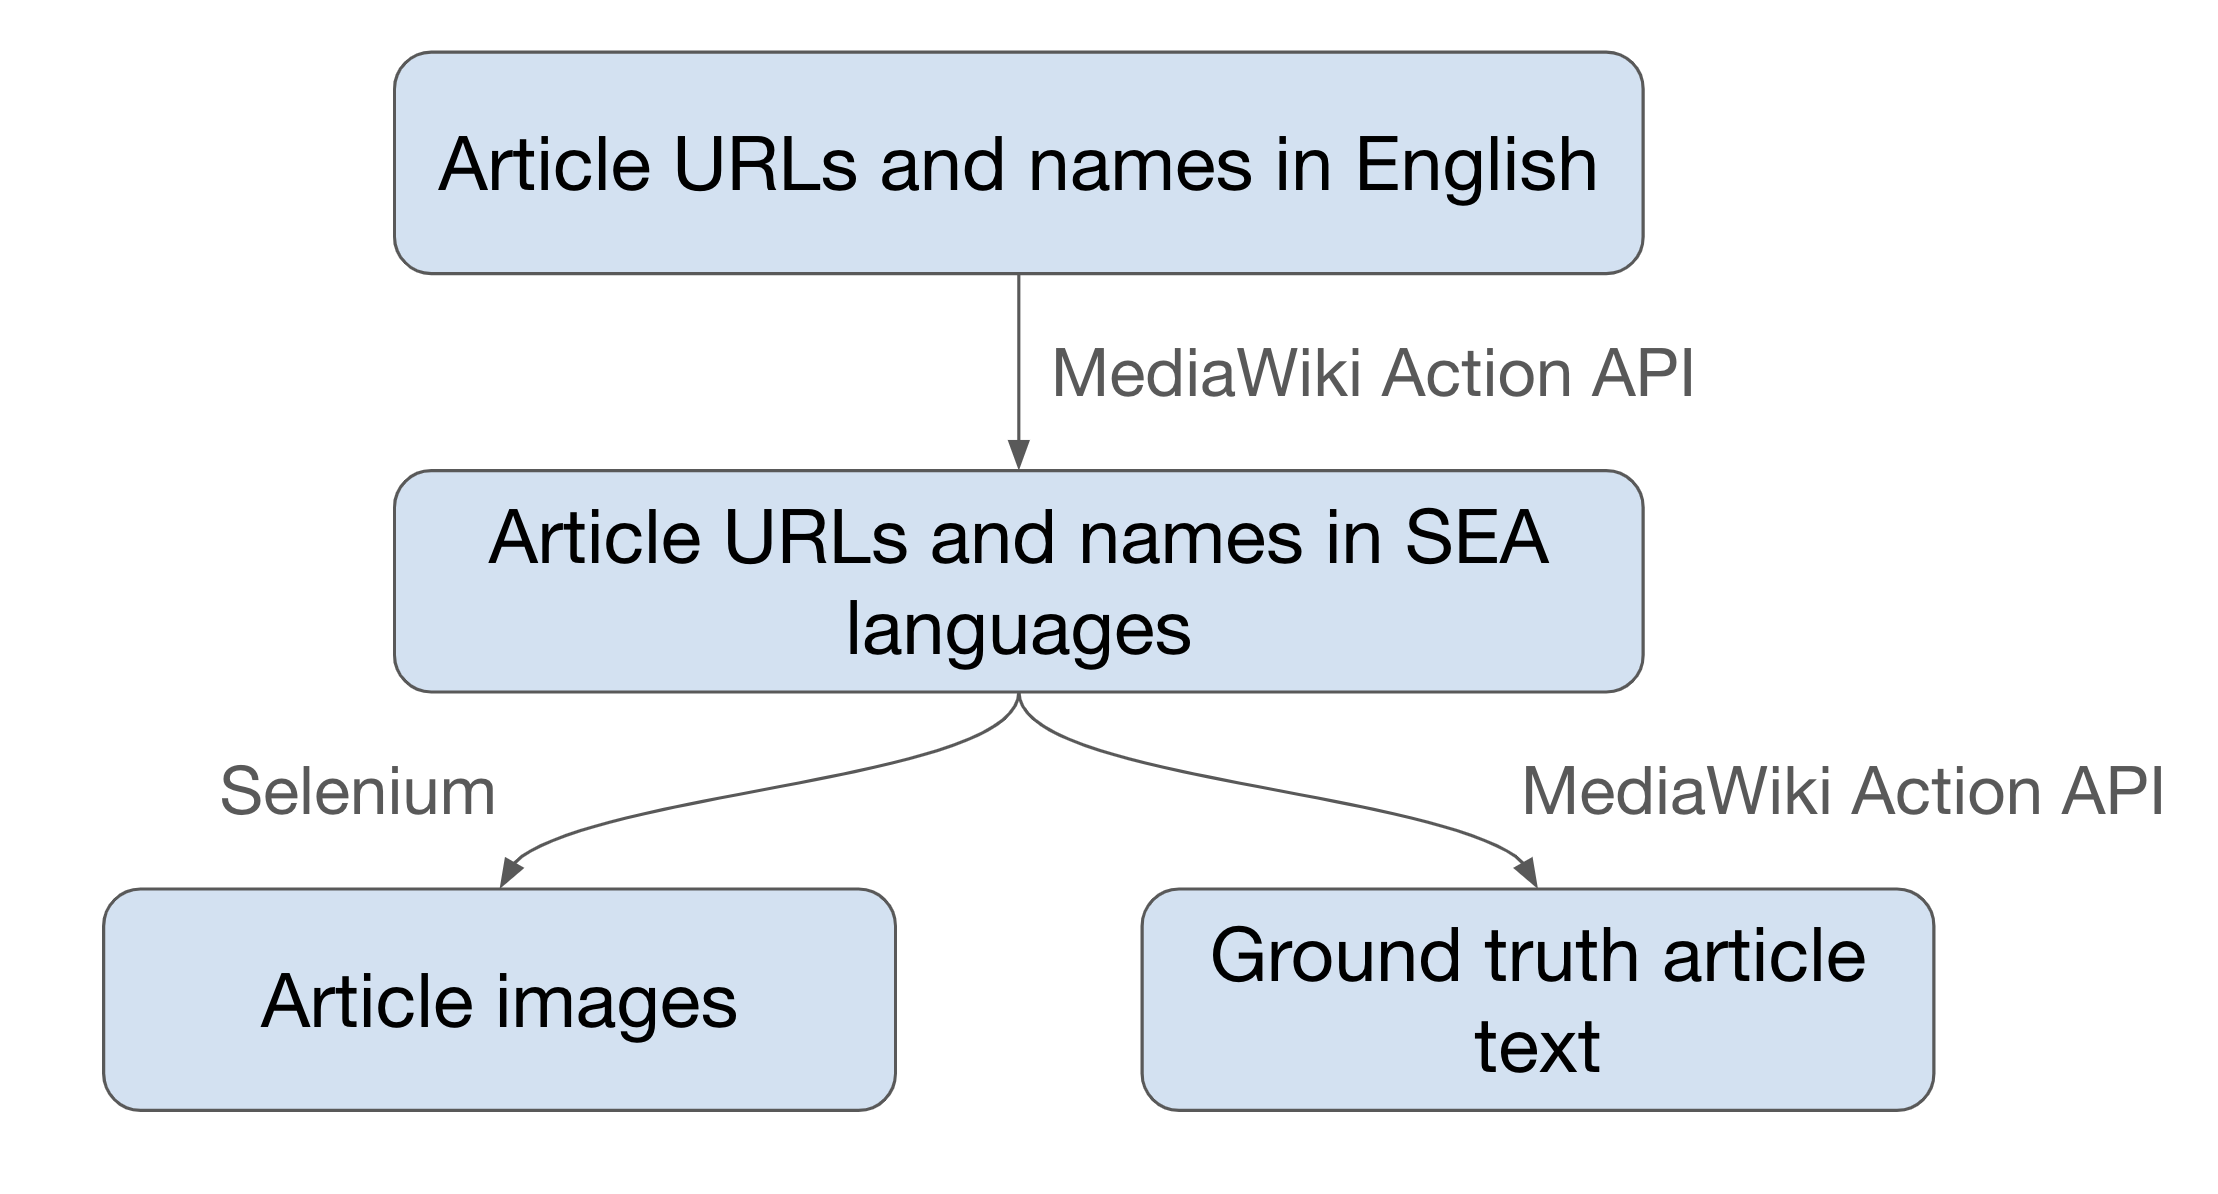
\includegraphics[width=0.6\textwidth]{images/data-collection.png}
    \caption{Pipeline for data collection from Wikipedia}
    \label{figure:data-collection}
\end{figure}

From the dataset of 100 Wikipedia articles, we collected article images and ground 
truth article text in our selected languages using Python, 
Selenium\footnote{\href{https://selenium-python.readthedocs.io}{Selenium} is a 
framework for automating web browsers, commonly used for web scraping by programmatically 
interacting with websites.}, and the MediaWiki Action API\footnote{The \href{https://www.mediawiki.org/wiki/API:Main_page}{MediaWiki Action API} allows 
access to wiki page operation features such as search and retrieval.}. Figure \ref{figure:data-collection} illustrates the overall pipeline 
for data collection. The detailed steps are as follows:

\begin{enumerate}
    \item Manually compile the dataset’s article names and URLs in English.
    \item Fetch the article names and URLs in Thai, Vietnamese, and Indonesian from the MediaWiki Action API.
    \item Download the article PDFs in all languages using Selenium.
    \item Convert the article PDFs into PNG images, where each image represents one page in the PDF.
    \item Download the ground truth article text into TXT files from the MediaWiki Action API.
\end{enumerate}

\section{Experiment 2: Benchmarking on Synthetic Data}

\subsection{Synthetic Data Generation}

\section{Experiment 3: Fine-tuning for Vietnamese and Thai}

\chapter{Results and Analysis}

In this chapter, we analyze and evaluate the results of the experiments to provide answers to the research questions.

\section{RQ1: How do popular OCR tools perform on SEA scripts?}

\subsection{OCR Accuracy}

\subsection{Runtime}

\begin{table}[ht]
    \caption{Average OCR Runtime Per Page (Seconds)}
    \label{table:runtime}
    \centering
    \begin{tabular}{lccc}
        \toprule
        & EasyOCR & Tesseract & GOT\\ 
        \midrule
        English & 3.23 & 11.68 & 24.35\\
        Indonesian & 2.92 & 13.19 & 31.44\\
        Vietnamese & 3.91 & 11.80 & -\\
        Thai & 2.32 & 16.76 & -\\
        \bottomrule
    \end{tabular}
\end{table}

\section{RQ2: What script-related challenges affect OCR accuracy on SEA languages?}

\begin{table}[ht]
    \caption{Error Classification by Character Type for English Articles}
    \label{table:english-error-classification}
    \centering
    \begin{tabular}{lrrrr}
        \toprule
        & \multirow{2}{*}{Count} & EasyOCR & Tesseract & GOT\\
        & & \% Missed & \% Missed & \% Missed\\
        \midrule
        Arabic digit & 38,324 & 0.7\% & 1.9\% & 0.3\%\\
        Latin letter & 1,546,964 & 1.3\% & 1.8\% & 0.4\%\\
        Latin letter w/ diacritic & 424 & 100.0\% & 53.1\% & 14.6\%\\
        Punctuation & 53,403 & 28.4\% & 2.3\% & 3.4\%\\
        Whitespace & 317,587 & 4.9\% & 4.3\% & 3.6\%\\
        Other & 3,298 & 82.8\% & 68.5\% & 76.9\%\\
        \bottomrule
    \end{tabular}
\end{table}

\begin{table}[ht]
    \caption{Error Classification by Character Type for Indonesian Articles}
    \label{table:indonesian-error-classification}
    \centering
    \begin{tabular}{lrrrr}
        \toprule
        & \multirow{2}{*}{Count} & EasyOCR & Tesseract & GOT\\
        & & \% Missed & \% Missed & \% Missed\\
        \midrule
        Arabic digit & 24,947 & 0.4\% & 1.8\% & 0.2\%\\
        Latin letter & 1,208,707 & 0.5\% & 1.8\% & 0.4\%\\
        Latin letter w/ diacritic & 262 & 5.3\% & 100.0\% & 15.3\%\\
        Punctuation & 37,788 & 22.1\% & 3.1\% & 0.8\%\\
        Whitespace & 207,556 & 4.8\% & 5.1\% & 4.1\%\\
        Other & 2,468 & 72.2\% & 80.5\% & 43.2\%\\
        \bottomrule
    \end{tabular}
\end{table}

\begin{table}[ht]
    \caption{Error Classification by Character Type for Vietnamese Articles}
    \label{table:vietnamese-error-classification}
    \centering
    \begin{tabular}{lrrr}
        \toprule
        & \multirow{2}{*}{Count} & EasyOCR & Tesseract\\
        & & \% Missed & \% Missed\\
        \midrule
        Arabic digit & 31,473 & 1.1\% & 2.2\%\\
        Latin letter & 916,667 & 8.5\% & 1.8\%\\
        Latin letter w/ diacritic & 292,686 & 14.8\% & 1.8\%\\
        Punctuation & 40,420 & 24.6\% & 2.2\%\\
        Whitespace & 367,936 & 10.9\% & 5.3\%\\
        Other & 35,767 & 12.5\% & 7.7\%\\
        \bottomrule
    \end{tabular}
\end{table}

\begin{table}[ht]
    \caption{Error Classification by Character Type for Thai Articles}
    \label{table:thai-error-classification}
    \centering
    \begin{tabular}{lrrr}
        \toprule
        & \multirow{2}{*}{Count} & EasyOCR & Tesseract\\
        & & \% Missed & \% Missed\\
        \midrule
        Arabic digit & 22,580 & 0.9\% & 6.7\%\\
        Latin letter & 36,174 & 100.0\% & 100.0\%\\
        Latin letter w/ diacritic & 96 & 100.0\% & 100.0\%\\
        Thai letter & 617,699 & 0.4\% & 3.1\%\\
        Thai diacritic & 90,620 & 3.7\% & 3.6\%\\
        Punctuation & 13,669 & 6.4\% & 8.4\%\\
        Thai punctuation & 901 & 78.8\% & 3.9\%\\
        Whitespace & 58,164 & 37.5\% & 37.2\%\\
        Other & 306,647 & 2.2\% & 7.1\%\\
        \bottomrule
    \end{tabular}
\end{table}

\section{RQ3: What techniques and recommendations can enhance OCR accuracy on SEA languages?}

\chapter{Discussion}

\chapter{Conclusion}

\printbibliography[title={References}]

\clearpage
\appendix
\renewcommand{\chaptername}{Appendix}

\chapter{Wikipedia Article Dataset}

\begin{table}[ht]
    \centering
    \begin{tabular}{p{1in}p{3.8in}}
        \toprule
        \textbf{Category} & \textbf{Articles} \\
        \midrule
        People & Elizabeth II, Barack Obama, Michael Jackson, Elon Musk, Lady Gaga, Adolf Hitler, Eminem, Lionel Messi, Justin Bieber, Freddie Mercury, Kim Kardashian, Johnny Depp, Steve Jobs, Dwayne Johnson, Michael Jordan, Taylor Swift, Stephen Hawking, Kanye West, Donald Trump\\
        \midrule
        Present countries & United States, India, United Kingdom, Canada, Australia, China, Russia, Japan, Germany, France, Singapore, Israel, Pakistan, Philippines, Brazil, Italy, Netherlands, New Zealand, Ukraine, Spain\\
        \midrule
        Cities & New York City, London, Hong Kong, Los Angeles, Dubai, Washington, D.C., Paris, Chicago, Mumbai, San Francisco, Rome, Monaco, Toronto, Tokyo, Philadelphia, Machu Picchu, Jerusalem, Amsterdam, Boston\\
        \midrule
        Life & Cat, Dog, Animal, Lion, Coronavirus, Tiger, Human, Dinosaur, Elephant, Virus, Horse, Photosynthesis, Evolution, Apple, Bird, Mammal, Potato, Polar bear, Shark, Snake\\
        \midrule
        Buildings and structures & Taj Mahal, Burj Khalifa, Statue of Liberty, Great Wall of China, Eiffel Tower, Berlin Wall, Stonehenge, Mount Rushmore, Colosseum, Auschwitz concentration camp, Great Pyramid of Giza, One World Trade Center, Empire State Building, White House, Petra, Large Hadron Collider, Hagia Sophia, Golden Gate Bridge, Panama Canal, Angkor Wat\\
        \bottomrule
    \end{tabular}
    \caption{Dataset of 98 Wikipedia articles}
    \label{table:dataset}
\end{table}

\end{document}
